\subsection[Konfiguracja urządzenia wykonującego (Michał Krakowiak)]{Konfiguracja urządzenia wykonującego}
\textit{W tym rozdziale można całkiem sporo napisać o usb gadget configfs, nie ma takich rzeczy w programie studiów, a wykorzystaliśmy to do skonfigurowania rpi0 do działania jako klawiatura, tu też zabrakło w tym tygodniu czasu, żeby rozpisać}
Uzyskanie zamierzonego efektu wymaga odpowiedniego oprogramowania pożądanej funkcjonalności oraz wcześniejszego skonfigurowania urządzenia wykonującego. Wszystkie urządzenia wykonujące przynależące do realizowanego systemu działają pod kontrolą dedykowanej dystrybucji systemu operacyjnego Linux. Umożliwia do sprawdzenie problemu konfiguracji do skorzystania z istniejących interfejsów jądra systemu operacyjnego służących do tworzenia tzw. gadżetów USB. 
Termin gadżet USB używany jest do określenia urządzenia posiadającego własny kontroler urządzenia USB (ang. USB device controller, UDC) oraz możliwość podłączenia do hosta USB w celu udostępnienia mu pewnych dodatkowych funkcjonalności. Skonfigurowane w ten sposób urządzenie rozpoznawane jest przez hosta jako zbiór konfiguracji, z których każda zawiera interfejsy (nazywanych też funkcjami). System operacyjny linux dostarcza wielu gotowych funkcji urządzeń USB np. obsługę protokołu HID.
Realizowana konfiguracja korzysta z interfejsu USB Gadget Configfs, który pozwala na definiowanie konfiguracji i funkcjonalności złożonych gadżetów USB (czyli takich, które mogą udostępniać więcej niż jedną funkcjonalność) z poziomu przestrzeni adresowej użytkownika i nie wymaga realizacji własnych modułów jądra systemu operacyjnego.
Aktywacja interfejsu USB gadget configfs wymaga załadowania dodatkowego modułu jądra:
\begin{lstlisting}[language=bash,caption={Ładownie modułu jądra do obsługi USB gadget configfs}]
    sudo modprobe libcomposite
\end{lstlisting}
Proces kreowania nowego urządzenia polega na wykonaniu poszczególnych operacji na plikach w nowo zamontowanym katalogu
\begin{table}[H]
    \begin{tabular}{|l|r|}
        \hline
        \textbf{Akcja} & \textbf{Operacja na systemie plików} \\
        \hline
            Stworzenie gadżet/funkcję/konfigurację & Stworzenie katalogu \textit{(mkdir)}\\
        \hline
            Usunięcie gadżet/funkcję/konfigurację & Usunięcie katalogu \textit{(rmdir)}\\
        \hline
            Ustawienie wartość atrybutu & Zapis do pliku \textit{(echo)}\\
        \hline
            Pobranie wartości atrybutu & Odczyt zawartości pliku \textit{(cat)}\\
        \hline
            Grupowanie funkcjonalności & Dowiązanie symboliczne \textit{(ln -s)}\\
        \hline
            Usunięcie grupy funkcjonalności & Usunięcie dowiązania symbolicznego \textit{(rm)}\\
        \hline    
    \end{tabular}
    \caption{Mapowanie operacji usb gadget configfs}  
    \label{tab:configs_map}
\end{table}
Działanie mechanizmu przedstawia \ref{fig:configfs}
\begin{figure}[H]
    \centering
    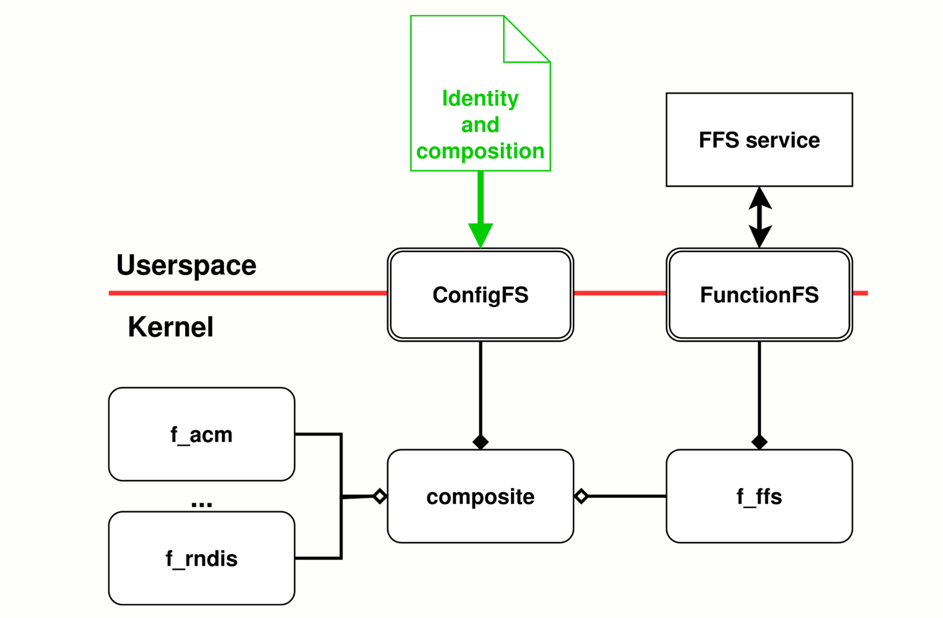
\includegraphics[width=\textwidth]{mk01}
    \caption{Configfs \cite{samsung}}
    \label{fig:configfs}
\end{figure}
